\chapter{Einleitung}

\section{Motivation}
\label{sec:Motivation}
\paragraph{}
Wenn man im Web nach einem Begriff sucht, kann die Suchanfrage nicht immer sofort genau definiert werden, besonders wenn das Thema der Suche dem Benutzer nicht bekannt ist. Um eine korrekte Anfrage aufbauen zu können, die die gewünschte Ergebnisse liefert, braucht man üblich mehr Iterationen - mit jeder Iteration wird die Anfrage präzisiert und verbessert. Da moderne Suchmaschinen allerdings keine strukturierte Informationen über die Suchergebnisse und auf der Suchergebnisseiten vorhandene Entitäten liefern, wird der Benutzer gezwungen, sich jedes Dokument manuell anzuschauen, um die Anregungen für neue Suchiterationen zu gewinnen, was als Folge zu einer niedrigen Arbeitsleistung führt.

Ein Beispiel für angesprochenes Problem ist auf der Abbildung \ref{fig:bing-issue} zu sehen. Man muss sich jeden gefundenen Snippet angucken und gelegentlich auch die gefundene Webseite öffnen, um die Antwort auf gestellte Frage zu erfahren, was bei längeren Suchsitzungen viel Zeit in Anspruch nimmt.

\begin{figure}
\centering
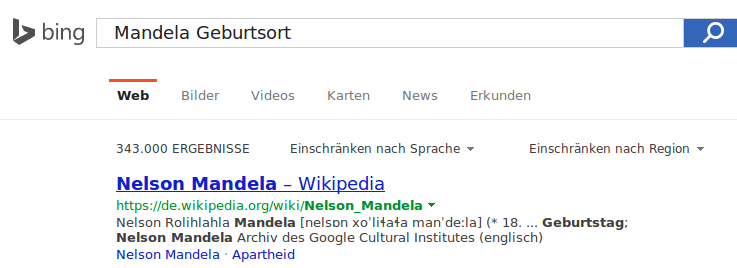
\includegraphics[width=1\textwidth]{Bilder/bing-search1.png}
\caption{''Eine Websuche ohne Extraktion von Entitäten''}
\label{fig:bing-issue}
\end{figure}

Es existieren bereits mehrere Einsätze, die den Benutzer bei der Suche und bei der Präzision seiner Suchanfragen unterstützen und die die Websuche beschleunigen können:
\begin{itemize}
\item Personalisierung der Suche\cite{noll2007web} - es wird versucht, mithilfe von Suchhistorie des Benutzers, seines Verhaltens im Netz oder seinen ,,Likes``-Einträgen in sozialen Netzwerken die Ergebnisse, die für diesen Benutzer relevant wären, ,,vorherzusagen`` und den entsprechenden Dokumenten ein höheres Gewicht bei der Suche zu geben.
\item Automatische Vervollständigung der Anfrage - sobald man anfängt den Text der Anfrage zu tippen, werden dem Benutzer Vorschläge bezüglich des Restes der Anfrage gemacht.
\item Autokorrektur der Anfrage - falls es keine Dokumenten gefunden wurden, könnte die Anfrage bei Bedarf automatisch korrigiert werden.
\end{itemize}

In Rahmen dieser Arbeit soll ein anderer Einsatz implementiert und erforscht werden: die Extraktion von Entitäten aus Suchergebnissen. 

Eine Skizze der erwähntes Einsatzes ist auf der Abbildung \ref{fig:bing-and-entity} zu sehen. Die Idee dieses Einsatzes besteht daran, dass dem Benutzer zusätzlich zu den Links die Liste von sogenannten Entitäten - Personen, Firmen oder geographischen Objekten - angezeigt wird, die aus den Snippets (kurzen Textausschnitten der gefundenen Webseiten) extrahiert wurden. Der Einsatz könnte die Suche beschleunigen, da der Benutzer im besten Fall die verlinkte Dokumente gar nicht mehr öffnen muss, sondern sich lediglich die extrahierte Entitäten anschauen muss.

\begin{figure}
\centering
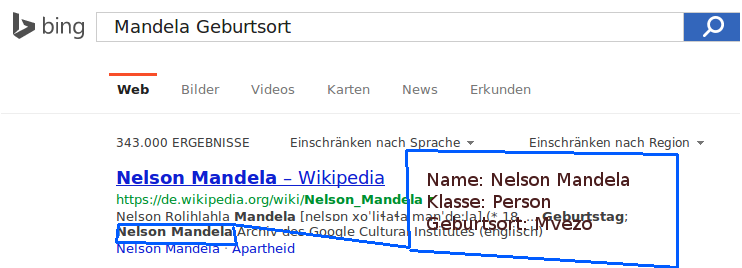
\includegraphics[width=1\textwidth]{Bilder/bing-and-entity1.png}
\caption{''Eine Websuche mit Extraktion von Entitäten''}
\label{fig:bing-and-entity}
\end{figure}

\section{Problemstellung}
\label{sec:Problemstellung}
\paragraph{}
Die Implementierung solches Einsatzes bringt mit sich allerdings bestimmte Herausforderungen, die im Rahmen dieser Arbeit angegangen werden müssen:

Die erste Frage wäre, wie genau kann man Entitäten in einem menschlichen Text überhaupt erkennen lassen. Können dazu feste Muster definiert werden, oder wäre der Einsatz von der Methoden aus künstlicher Intelligenz notwendig? Gibt es schon Algorithmen, die Entitäten erkennen können, oder müssen eigene kreiert werden? 

Zweitens, es ist nicht klar, ob die kurze Textsnippets, die die Suchmaschinen liefern, für die Extraktion von Entitäten überhaupt benutzt werden können - das Problem ist, dass diese Textabschnitte sehr klein (üblicherweise zwei bis drei Sätze) sind, und es ist durchaus möglich, dass die gar keine Entitäten beinhalten.

Außerdem kann der zusätzliche Schritt der Erkennung von Entitäten kann große Verzögerungen in die Suche bringen, was die Nutzbarkeit dieses Einsatzes zunichte machen könnte, wenn die Suche viel länger dauern wird, als die ohne der Extraktion von Entitäten.

Eine weitere Herausforderung wäre, dass jede natürliche Sprache ein besonderes an diese Sprache angepasstes Verfahren braucht, um erkennen zu können, welche Entitäten in dem Text vorkommen. Für englische Sprache existieren schon jetzt Verfahren und Modellen, mit deren Hilfe die englischsprachige Entitäten extrahiert werden können. Allerdings fehlt solches Modell für die deutsche Sprache, deswegen findet die Extraktion von deutschsprachigen Entitäten zurzeit nicht statt.

Zusätzlich zu den oben genannten Herausforderungen kann man folgendes Problem, das sich als eine getrennte Unteraufgabe definieren lässt, erkennen: wenn man dem Benutzer \textbf{nur} die Entitäten zeigt, ohne dazugehörigen Daten wie Geburtsort, Todesdatum oder Muttersprache, wird solcher Einsatz für den Benutzer kaum nützlich sein können. Deswegen sollen für die im Text erkannte Entitäten auch die dazugehörige Informationen extrahiert werden. Dieser Schritt nennt man ,,Verlinkung`` von Ontologien (eine Darstellung von ,,Wissen`` über ein Objekt), weil hier die Entität mit den Daten aus einer Datenbank verlinkt werden.

Bei der Verlinkung von Entitäten soll folgendes im Kauf genommen werden:
\begin{itemize}
\item In welcher Datenbank soll nach Informationen über eine Entität gesucht werden? Wo findet man die Daten?
\item Wird die Geschwindigkeit der Suche durch Verlinkung stark beeinträchtigt?
\item Was macht man, wenn der Name der Entität im Text mit in der Datenbank vorhandenen Namen nicht übereinstimmt? Wie wählt man den am besten passenden Datenbankeintrag? Wie wird die Suche generell durchgeführt?
\end{itemize}

Aber auch wenn alle Entitäten aus dem Text extrahiert wurden, hat man das Problem, dass einige Entitäten ,,irrelevant`` sein könnten. Solche Entitäten, die dem Benutzer nicht weiter helfen können, sollen bei Möglichkeit rausgefiltert werden, damit die dem Benutzer nicht angezeigt werden. 

Damit die Extraktion von Entitäten auch in Drittaplikationen wie Websuche-Gamifikation-Apps\cite{Karatassis:15} integriert werden könnte, muss nachgedacht werden, wie für den Entwickler am besten passende API implementiert werden könnte.

Eine andere Frage wäre, wie kann die Effizienz dieses Einsatzes beurteilt werden? Wie kann festgestellt werden, ob die Extraktion von Entitäten aus Suchergebnisseiten für den Benutzer hilfreich sein könnte?

Alle diese Fragen sollen im Rahmen dieser Arbeit angegangen und gegebenenfalls gelöst werden.

\section{Aufgabenstellung}
\label{sec:Aufgabenstellung}
\paragraph{}
Nachdem die Ziele dieser Arbeit definiert wurden, können die dazugehörige Abschnitte genauer definiert werden: 
\begin{itemize}
\item Es soll ein Framework entwickelt werden, das die Extraktion von Entitäten aus deutschsprachigen Texten ermöglicht:
\begin{enumerate}
\item Zuerst sollen Algorithmen zur Extraktion von Entitäten aus Texten erforscht werden.
\item Danach soll auf Basis von diesen Algorithmen die Extraktion von Entitäten aus Texten implementiert werden.
\item Die irrelevante Entitäten sollen rausgefiltert werden (es soll außerdem definiert werden, wie eine ,,unwichtige`` Entität bestimmt wird).
\item Es soll gegebenenfalls eine Applikation für Training von Extraktionsmodellen implementiert werden, falls noch keine vorhanden ist.
\item Im letzten Unterschritt soll die passende Datenquelle ausgewählt und die Verlinkung von Daten aus dieser Datenbank mit im vorherigen Schritt extrahierten Entitäten implementiert werden 
\end{enumerate}

\item Danach soll eine Bibliothek entwickelt werden, die dem Entwickler einfache API zur Anreicherung von Suchergebnissen zur Verfügung stellt. Der Entwickler soll idealerweise keine Wissen und Kenntnisse über Extraktion von Entitäten besitzen müssen - die Schnittstelle soll dabei im einfachsten Fall nur eine Funktion zur Verfügung stellen, die ein Suchsnippet als Eingabe und Liste von Ontologien (Namen und Eigenschaften von Entitäten) als Ausgabe verwendet.

\item Es soll anschließend eine Evaluierung durchgeführt werden, um feststellen zu können, ob aus den Suchergebnissen gewonnene Entitäten für den Benutzer tatsächlich relevant sind. Außerdem soll die Evaluierung die in der Sektion \ref{sec:Problemstellung} gestellte Fragen zu beantworten helfen können. Zusätzlich dient dieser Schritt zum Austesten der entwickelten API, die in der Evaluierungsapplikation eingesetzt werden soll.
\end{itemize}